%-----------------------------------------------------------------------------------------------------
\chapter{State of the Art}
\label{cap2:State_Of_The_Art}
%-----------------------------------------------------------------------------------------------------

%-----------------------------------------------------------------------------------------------------
\section{Introduction}
%-----------------------------------------------------------------------------------------------------

Over the last few decades, technology has advanced rapidly, especially in telecommunications. Antennas have a crucial role in this context as they are key elements in the communication chain, upon which the overall performance of the system strongly depends. Since World War I, the design and development of antennas has been a topic of great relevance, initially driven by military applications. Over time, this importance has increased with the introduction of new technologies, such as television, and continues to grow in the current era of mobile communications, including 5G and high-frequency Wi-Fi. The need to characterize and evaluate an antenna's performance has become even more crucial to ensure the efficiency and reliability of communication systems.


To ensure that antennas operate within expected parameters, it is essential to use measurement and calibration systems. These systems allow the evaluation of various antenna characteristics, including radiation pattern, gain, efficiency, and bandwidth. Measuring and validating antenna performance is vital to make sure they meet technical and regulatory specifications.


Radiation pattern measurement is a key step in the design process of antennas and wireless devices. The results of these measurements are used to validate simulated designs and identify potential performance issues before final testing.


While commercially available antenna measurement systems are designed to provide precise and repeatable measurements, they are often expensive. Therefore, custom-made solution are the way when budget is a constraint. These custom-made solutions offer a cost-effective alternative, while addressing specific needs that commercial systems may not cover.

In this chapter, some available commercial solutions for antenna radiation patterns measurement will be first presented. Then, a review is made regarding research and development works that aim to develop similar devices. The goal is to provide a theoretical and practical basis that supports the decision to develop an cost-effective and accurate solution, aligning with the objectives of this project.

%-----------------------------------------------------------------------------------------------------
\section{Commercially Available Products}
\label{cap2:sec2:Commercially Available Products}
%-----------------------------------------------------------------------------------------------------

This section presents commercially available solutions for measuring antenna radiation patterns. These solutions are used in research and development laboratories as well as in companies that need to validate antenna performance across different frequencies. The following descriptions provide a detailed overview of the main features and the purpose for which each system is most suitable. It should be noted that the list presented is not exhaustive and only includes companies that were contacted as part of this study.


\subsection{MegiQ RMS-0460}

According to the supplier, the MegiQ RMS-0460 system, manufactured in the Netherlands, is designed to perform antenna radiation pattern measurements in environments such as laboratories or offices, without requiring an anechoic chamber, as shown in Figure \ref{cap2:sec2:fig1}. It operates over a frequency range of 370 MHz to 6 GHz and supports measurements along three axes. The system offers a measurement accuracy of $\pm 1$ dB and repeatability of $\pm 0.5$ dB. Depending on the configuration, the system can handle loads up to 30 kg. The approximate price is \euro\;16,950.


\begin{figure}[H]
    \centering
    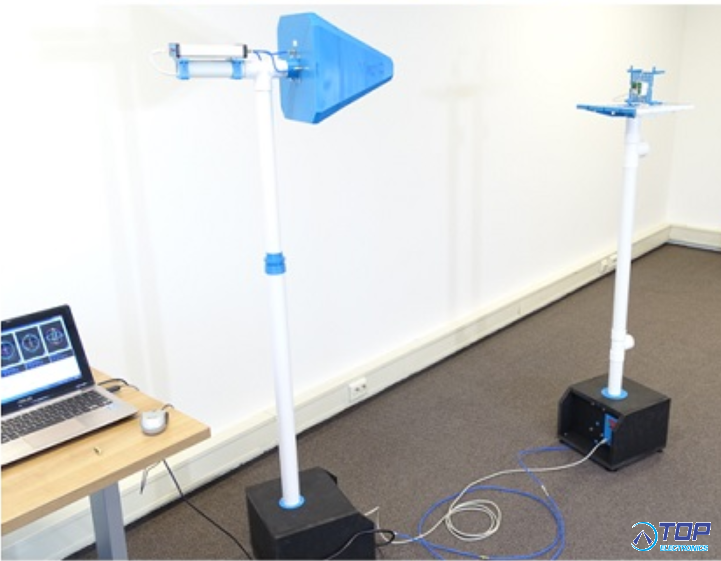
\includegraphics[scale=0.8]{Imagens/MegiQ RMS-0460.png}
    \caption{MegiQ RMS-0460 Measurement System.}
    \label{cap2:sec2:fig1}
    
    \vspace{2mm} % Espaço entre legenda e a fonte
    \small \textit{Source: MegiQ, 2024.} % Fonte da imagem
\end{figure}



\subsection{D6050 Diamond Engineering}

The D6050, produced by Diamond Engineering in the United States, is designed to perform measurements over a frequency range up to 67 GHz, and up to 110 GHz when using waveguides. It offers an angular precision of $0.02^\circ$ and supports loads up to 11.5 kg. The system, depicted in Figure \ref{cap2:sec2:fig2}, features a modular configuration that allows the addition of linear axes for automated measurement. Additionally, it includes software for control and data analysis. The starting price is \euro\;12,880.

\begin{figure}[H]
    \centering
    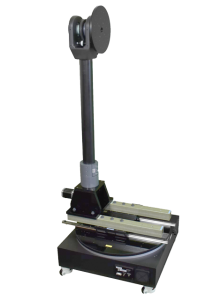
\includegraphics[scale=1.2]{Imagens/D6050.png}
    \caption{D6050 Measurement System.}
    \label{cap2:sec2:fig2}
    
    \vspace{2mm} % Espaço entre legenda e a fonte
    \small \textit{Source: Diamond Engineering, 2024.} % Fonte da imagem
\end{figure}




\subsection{Microwave Factory Co., Ltd. (MWF)}

Microwave Factory Co. Ltd., from Japan, offers an option for measuring antenna radiation patterns, operating in a range from 0.4 GHz up to 300 GHz, depending on the configuration. As shown in Figure \ref{cap2:sec2:fig3}, the system includes an antenna tower, azimuth positioner, elevator, RF absorbers, and control software (MATEOS.NET), enabling 2D radiation pattern measurements and antenna gain analysis. The system is customizable to accommodate equipment with varying weights, with a capacity of up to 1000 kg, which allows it to be used for large-scale projects in controlled environments. It offers an angular precision of $0.03^\circ$ and repeatability of $\pm 0.03^\circ$. However, it requires an anechoic chamber to ensure measurement accuracy. The total price for the complete system is approximately \euro\;368,000.

\begin{figure}[H]
    \centering
    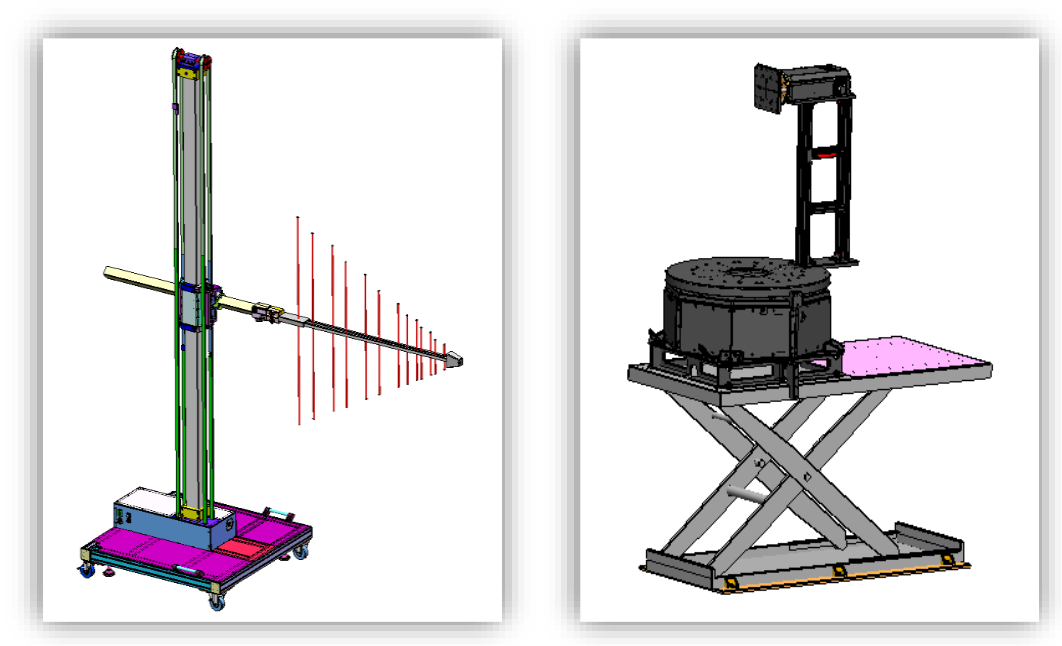
\includegraphics[width=\textwidth]{Imagens/MWF.png}
    \caption{Microwave Factory (MWF) Measurement System representation.}
    \label{cap2:sec2:fig3}
    
    \vspace{2mm} % Espaço entre legenda e a fonte
    \small \textit{Source: Microwave Factory Co. Ltd., 2024.} % Fonte da imagem
\end{figure}


\subsection{S7601A Antenna Measurement System}

The S7601A Antenna Measurement System, developed by Keysight Technologies, a United States company, is also a product for antenna characterization. It operates within a frequency beginning from 10 MHz to 50 GHz and allows for both near-field and far-field measurements. This system supports 2-axis positioning and can handle antennas weighing up to 10 kg. According to the manufacture, it enable measurement accuracy up to $\pm 0.8$ dB, delivering results for various antenna systems, including 5G, satellite, and radar applications. The system includes an integrated anechoic chamber, which, for reference, the price of the S7601A anechoic chamber alone is approximately \euro\;856,000. Additional measurement devices are offered by the same company and can be acquired based on the specific needs of the user. The system is illustrated in Figure \ref{cap2:sec2:fig4}.


\begin{figure}[H]
    \centering
    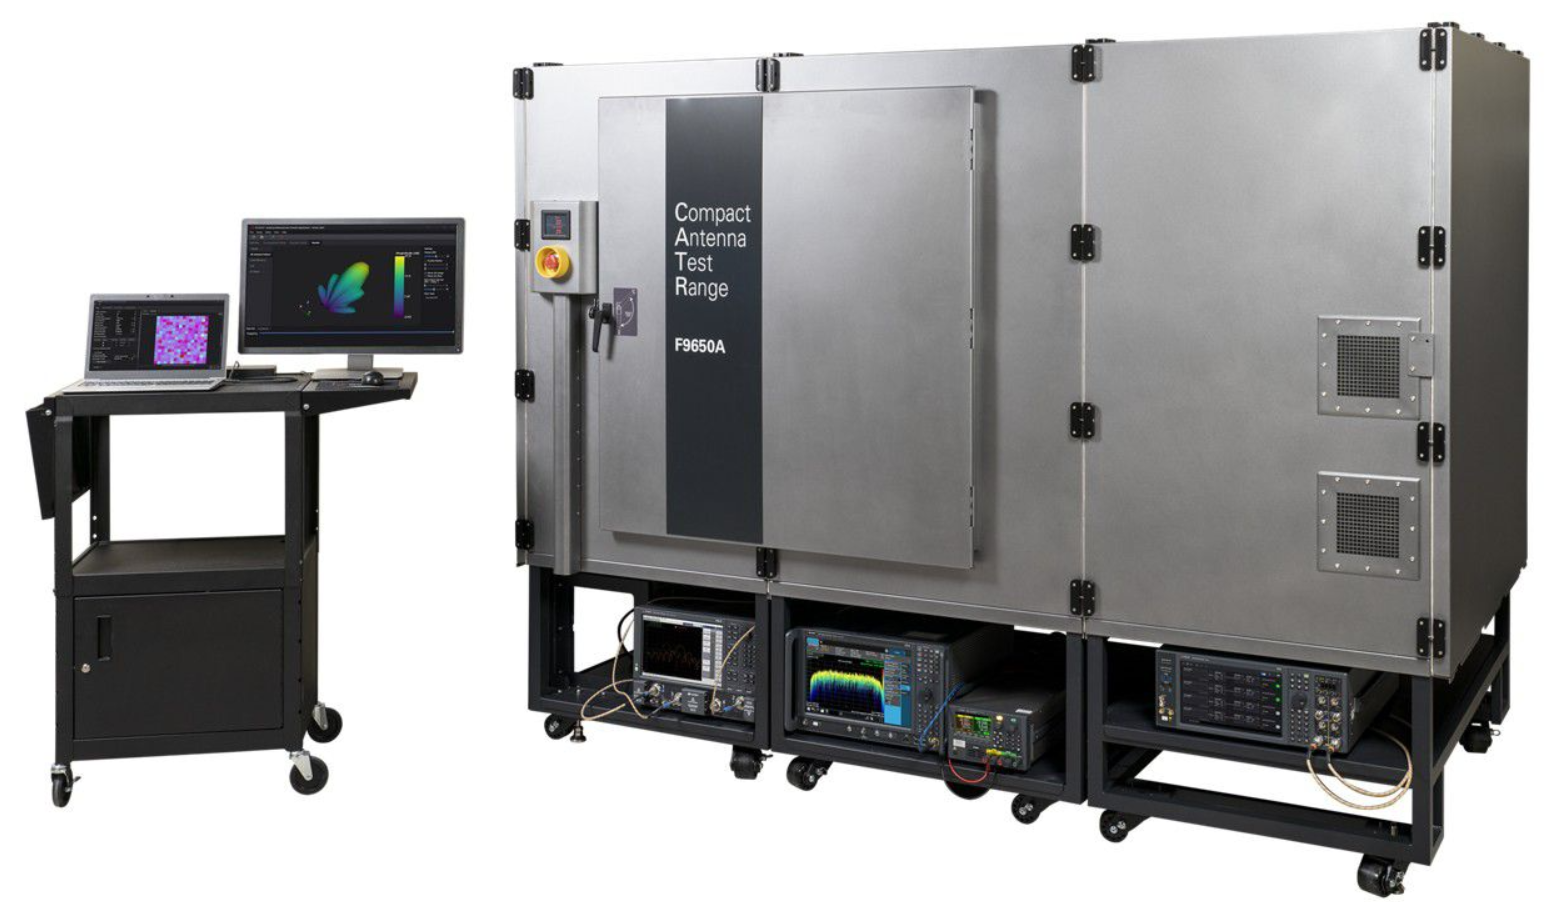
\includegraphics[scale=0.45]{Imagens/S7601A.png}
    \caption{S7601A Antenna Measurement System.}
    \label{cap2:sec2:fig4}
    
    \vspace{2mm} % Espaço entre legenda e a fonte
    \small \textit{Source: Keysight Technologies, 2024.} % Fonte da imagem
\end{figure}


As referred in the beginning of this section, contact was made via email with the companies that manufacture these systems. Despite this, some specific information regarding certain features, such as signal accuracy or load capacity, was either not provided or is not applicable due to possible configurations of the system. This explains the gaps in the comparison provided in Table \ref{cap2:sec2:table1} where data is unavailable or subject to change based on client requirements.

\begin{table}[H]
\centering
\caption{Comparison of Commercial Antenna Measurement Systems}
\resizebox{\textwidth}{!}{%
\begin{tabular}{|l|l|l|l|l|}
\hline
\textbf{Feature}               & \textbf{MegiQ RMS-0460}   & \textbf{D6050 Diamond Eng.} & \textbf{Microwave Factory}   & \textbf{S7601A}             \\ \hline
\textbf{Frequency Range}       & 370 MHz – 6 GHz           & Up to 67 GHz (110 GHz)       & 0.4 GHz – 6 GHz            & 10 MHz – 50 GHz             \\ \hline
\textbf{Measurement Axes}      & 3-axis                    & 2-axis                      & 2-axis                       & 2-axis                      \\ \hline
\textbf{Signal Accuracy (dB)}  & $\pm 1$ dB                     & Not Specified               & Not Specified                & $\pm 0.8$ dB                     \\ \hline
\textbf{Angular Precision ($^\circ$)} & Not specified             & $0.02^\circ$                       & $0.03^\circ$                        & Customizable               \\ \hline
\textbf{Load Capacity}         & Up to 30 kg           & 11.5 kg                     & Up to 1000 kg                & 10 kg                       \\ \hline
\textbf{Environment}           & No chamber required       & No chamber required         & Needs chamber                & Chamber included            \\ \hline
\textbf{Price}                 & \euro\;16,950                   & \euro\;12,880                     & \euro\;368,000                     &  \euro\;856,000 (Chamber only)             \\ \hline
\end{tabular}%
}

\label{cap2:sec2:table1}
\end{table} \vspace{0.15cm}

In conclusion:
\begin{itemize}

\item The MegiQ RMS-0460 system is designed for smaller to medium-sized antennas, with a load capacity of up to 30 kg, depending on the configuration. It operates without requiring an anechoic chamber, making it applicable for environments like laboratories or educational settings, where portability and ease of setup are necessary.

\item The D6050 Diamond Engineering system provides an angular precision of $0.02^\circ$, suitable for applications that require accurate positioning of antennas. It operates within a frequency range up to 110 GHz when using waveguides, and supports high-frequency measurements for medium-sized antennas.

\item The Microwave Factory Co., Ltd. system has the highest load capacity among the compared systems, supporting up to 1000 kg. This makes it the choice for large-scale projects, such as those involving heavy or large antennas. It also provides a frequency range up to 300 GHz, making it suitable for advanced applications in aerospace or defence industries where high precision and anechoic chamber-controlled environments are critical.

\item The S7601A Antenna Measurement System has a load capacity of up to 10 kg and operates within a frequency range of 10 MHz to 50 GHz. It includes an integrated anechoic chamber, allowing measurements without the need for a separate chamber, making it applicable for industries such as telecommunications and satellite testing.

\end{itemize}

The baseline is that any of the solution, even the most cost-effective, is way outside the grasp of many educational institutions. For this reason, do-it-yourself (DIY) solutions provide the most practical approach. In this reference frame, the following section will be devoted to explore academic published researches that describe the development of custom-made antenna radiation pattern measurement rigs.

%-----------------------------------------------------------------------------------------------------
\section{Research and Development Work}
%-----------------------------------------------------------------------------------------------------

Based on the characteristics of the commercial equipment discussed above, it is possible to conclude that, even if they are highly effective and precise, they can also be quite expensive. For many individuals, organizations, and companies, the high costs of these systems may not be justifiable, especially when financial resources are limited.\\
\vspace{0.1em}
\indent As a result, custom-made solutions emerge as an alternative. These solutions allow for the construction of customized measurement systems that can focus on specific antenna characteristics without the need to acquire complete and expensive commercial systems. Additionally, these solutions can be adapted to include functionalities not covered by commercial systems, providing greater flexibility and cost savings.\\
\vspace{0.1em}
\indent \textbf{Research Methodology:} The literature review was conducted using two major academic databases: Google Scholar and IEEE Xplore (Institute of Electrical and Electronics Engineers Xplore). The search aimed to identify existing commercial antenna measurement systems, as well as academic and open-source solutions focusing on low-cost and customisable alternatives. A set of keyword combinations was used to ensure a comprehensive search, including: ``antenna measurement'', ``antenna measurement system'', ``radiation pattern'', ``automated antenna measurement'', ``low-cost antenna measurement'', ``open-source antenna measurement'', ``SDR antenna measurement'', ``Arduino antenna system'', and ``3D-printed antenna measurement''. Boolean operators such as AND were used to refine the queries (e.g., ``antenna measurement'' AND ``radiation pattern''; ``open-source antenna'' AND ``antenna measurement system'').\\
\vspace{0.1em}
\indent Picco and Martin (2011) developed ``An Automated Antenna Measurement System Utilizing Wi-Fi Hardware''. On their work a device was built using commercial Wi-Fi hardware\cite{6157745}. In particular, specifically modified Linksys brand? routers, to measure RF signals at 2.4 GHz. By replacing the original firmware with open-source DD-WRT firmware, they enabled the routers to function as cost-effective tools for measuring the received signal strength indicator (RSSI). Additionally, the system integrates with LabVIEW software to automate the positioning of the antenna under test using stepper motors. Although the system operates in a non-anechoic environment, the published results suggest that inaccuracies are kept controlled while providing a viable low-cost solution for educational and research settings.

In Junfithrana \textit{et al.} (2017), ``Development of Automated Antenna Radiation Pattern Measurement Using Rotator Application Model to Increase Accuracy'', the authors proposed an automated system that uses a two-axis rotator model controlled by microcontrollers\cite{8308101}. This setup is integrated with a vector network analyzer and the control software was developed in LabVIEW. The work highlights how the use of accessible components can increase measurement accuracy, making the system a practical and economical alternative to commercial solutions.

Simanjuntak \textit{ et al.} (2019), presents the ``Preliminary Design of Automatic Antenna Radiation Pattern Measurement System for Antenna and Propagation Laboratory Course'', in which the authors develop an automated radiation pattern measurement system using microcontrollers\cite{Simanjuntak2019/02}. This study demonstrates that an accessible and portable system can be implemented to be used in educational environments, providing quick and accurate measurements without the need for expensive commercial equipment.


All the above papers exemplify how custom solutions can be adapted to meet specific needs, offering an efficient alternative to commercial systems. They offer a solid foundation for developing new approaches that combine cost-effectiveness, flexibility, and innovation, which is aligned with the goal of this project.


Within the maker community, open-source solutions have gained prominence in the field of antenna measurement due to their flexibility, cost-effectiveness, and adaptability to different research and educational contexts. Examples of such approaches include the work developed by Weber State University, which proposed an antenna pattern measurement system using open-source components, such as Software-Defined Radios (SDRs), Arduino microcontrollers, and GNU Radio software. These studies present the continuous evolution and improvement of accessible and highly effective antenna measurement systems.


Also, in ``Open-Source Antenna Pattern Measurement Validation Using FEKO'' (2020) an antenna pattern measurement system developed using SDRs and 3D-printed hardware, is presented\cite{9196138}. The system validation was conducted by comparing experimental measurements of antenna radiation patterns with theoretical simulations generated by the FEKO simulation software. The results demonstrated that the low-cost system could replicate measurements with a high degree of accuracy, making it an ideal tool for undergraduate-level investigations on antenna theory and practical measurements.


In the same year, ``Open-Source Antenna Pattern Measurement System'' (2020) presents the development of a measurement system by replacing Wi-Fi routers with SDRs to expand the frequency range (30 MHz to 6 GHz) over which measurements can be performed\cite{9280870}. This enhanced version of the system addresses challenges related to position control and measurement accuracy, using stepper motors controlled by an Arduino with open-source GRBL firmware. The study highlights how the replacement of components and the integration of new control and signal processing methods helped improve the system's precision and versatility while keeping it accessible and suitable for educational environments.


Finally, the most recent work among the studies reviewed, "Open-Source Antenna Pattern Measurement System: SDR-based Student Research and Development" (2022)\cite{finger2022open}, presents the latest updates to the system, including significant hardware and software improvements. Hardware upgrades include replacing Polyvinyl Chloride (PVC) components with Computer-Aided Design (CAD)-modelled and 3D-printed parts, increasing the system's mobility and adaptability for use in multiple noisy environments. The software was enhanced with new versions of Python, GNU Radio, and Linux, and advanced noise mitigation techniques and modulation control were incorporated to further improve measurement accuracy. The article highlights the system's success as a robust and flexible educational tool, creating opportunities for collaborative research and project development among electrical engineering students.

